% ============================================================================
%  COMPILE WITH XeLaTeX  (twice, so the point total resolves)
%  Overleaf: Menu -> Compiler -> XeLaTeX
%  Requires: bnhandout.sty and fonts/Kalpurush.ttf in the project
% ============================================================================
\documentclass[11pt]{article}
\usepackage{bnhandout}
\usepackage{amsmath}

% add [nosol] for a student edition

\hauthor[https://sites.google.com/view/jugantordey/home]{Jugantor Dey}
\hseries{\textit{Mathematics for the Physics Olympiad}}

\begin{document}

\handouttitle{Chapter 21 : Vector Calculus}

\noindent
এটি সিরিজের শিখর। এখানে চারটি অধ্যায় একসঙ্গে কাজে লাগবে: ২০ (ভেক্টর,
dot ও cross product), ১৭ (integral), ১১ (solid angle ও ঘন জ্যামিতি) এবং
১২ (cylindrical ও spherical স্থানাঙ্ক)। সেই সঙ্গে ১৫ নম্বরের আংশিক
derivative আর ১৬ নম্বরের ক্ষুদ্র উপাদান ছাড়া এক পাতাও এগোনো যাবে না।

সিরিজজুড়ে অনেকগুলো ধার এখানে এসে শোধ হবে। ১১ নম্বর অধ্যায়ে solid angle
পরিচয় করিয়ে বলা হয়েছিল যে Gauss-এর সূত্র এর পরিণত রূপ; ১৫ নম্বরে বলা
হয়েছিল যে তিনটি আংশিক derivative একসঙ্গে একটি ভেক্টর বানায় যার নাম gradient;
১৬ নম্বরে $\mathbf{E}\cdot d\mathbf{a}$ ধরনের রাশির কথা বলা হয়েছিল;
১৯ নম্বরে বলা হয়েছিল যে PDE লেখার ভাষা এখানে তৈরি হবে। সবগুলোই এই
অধ্যায়ে।

মূল ধারণাটি একটি প্রতীক: $\nabla$। এটি একই সঙ্গে তিনটি কাজ করে, আর কোন কাজটি
করছে তা ঠিক হয় তার ডান পাশে কী বসেছে তার উপর। Scalar বসালে gradient,
ভেক্টরের সঙ্গে dot বসালে divergence, cross বসালে curl। তিনটি আলাদা ধারণা নয়,
একটিই বস্তু তিনটি টুপি পরে আছে।

আর তিনটি বড় উপপাদ্য একই কথা তিনভাবে বলে: \emph{ভেতরে যা ঘটছে তার যোগফল সমান
সীমানা দিয়ে যা পার হচ্ছে তার যোগফল}। ১৭ নম্বর অধ্যায়ের মৌলিক উপপাদ্যও
ঠিক এই কথাই বলত, কেবল এক মাত্রায়। এই অধ্যায়ে মোট \totalpoints\ পয়েন্ট
আছে।

\section{স্কেলার ও ভেক্টর ক্ষেত্র}

\begin{idea}[ক্ষেত্র]
স্থানের প্রতিটি বিন্দুতে যদি একটি সংখ্যা বসানো থাকে, তবে সেটি একটি
\emph{scalar field} $T(x,y,z)$। প্রতিটি বিন্দুতে যদি একটি ভেক্টর বসানো থাকে,
তবে সেটি একটি \emph{vector field}
$\mathbf{v}(x,y,z)$।
\end{idea}

উদাহরণ চারপাশেই আছে। ঘরের প্রতিটি বিন্দুর তাপমাত্রা একটি scalar field; বাতাসের
বেগ একটি vector field। তড়িৎ ক্ষেত্র $\mathbf{E}$, চৌম্বক ক্ষেত্র
$\mathbf{B}$, মহাকর্ষীয় ক্ষেত্র $\mathbf{g}$, সবই vector field। বিভব $V$ ও
চাপ $p$ scalar field।

ছবি আঁকার দুটি চেনা উপায়। Scalar field-এর জন্য সমমান রেখা বা তল (level
curve, level surface): যেসব বিন্দুতে $T$-এর মান সমান। Vector field-এর জন্য
প্রতিটি বিন্দুতে ছোট তীর, অথবা ক্ষেত্ররেখা।

\begin{center}
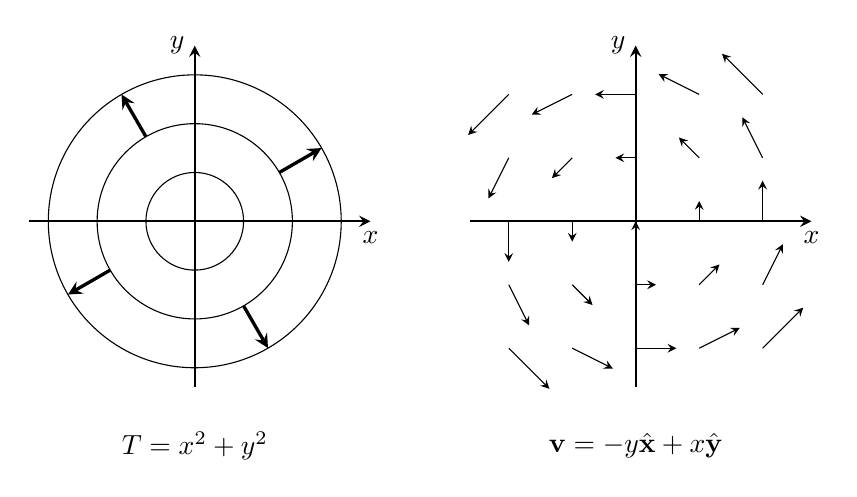
\begin{tikzpicture}[x=0.62cm,y=0.62cm,>=stealth]
 \begin{scope}
  \draw[thick,->] (-3.4,0) -- (3.6,0) node[below] {$x$};
  \draw[thick,->] (0,-3.4) -- (0,3.6) node[left] {$y$};
  \foreach \R in {1,2,3}{ \draw[thin] (0,0) circle (\R); }
  \foreach \a in {30,120,210,300}{
    \draw[very thick,->] (\a:2) -- (\a:3.0);
  }
  \node at (0,-4.6) {$T=x^{2}+y^{2}$};
 \end{scope}
 \begin{scope}[xshift=5.6cm]
  \draw[thick,->] (-3.4,0) -- (3.6,0) node[below] {$x$};
  \draw[thick,->] (0,-3.4) -- (0,3.6) node[left] {$y$};
  \foreach \i in {-2,-1,0,1,2}{
   \foreach \j in {-2,-1,0,1,2}{
    \pgfmathsetmacro\ux{-0.32*\j}
    \pgfmathsetmacro\uy{0.32*\i}
    \draw[->] (\i*1.3,\j*1.3) -- ++(\ux*1.3,\uy*1.3);
   }}
  \node at (0,-4.6) {$\mathbf{v}=-y\hat{\mathbf{x}}+x\hat{\mathbf{y}}$};
 \end{scope}
\end{tikzpicture}
\end{center}

বাঁ দিকের ছবিতে বৃত্তগুলো $T = x^{2}+y^{2}$-এর সমমান রেখা, আর মোটা তীরগুলো
পরের অনুচ্ছেদের gradient (একটু আগেই দেখিয়ে রাখলাম যে তারা সমমান রেখার উপর
লম্ব)। ডান দিকে একটি ঘূর্ণনশীল vector field।

\begin{example}
$T(x,y,z) = z$ এবং $T(x,y,z) = x^{2}+y^{2}+z^{2}$ ক্ষেত্র দুটির সমমান তল
বর্ণনা করো।
\end{example}

\begin{solbox}
প্রথমটি: $z = c$ মানে অনুভূমিক সমতল। সমমান তলগুলো একগুচ্ছ সমান্তরাল সমতল,
যেমন বায়ুমণ্ডলের চাপের আনুমানিক ছবি।

দ্বিতীয়টি: $x^{2}+y^{2}+z^{2} = c$ মানে $\sqrt{c}$ ব্যাসার্ধের গোলক
(১২ নম্বর অধ্যায়)। সমমান তলগুলো মূলবিন্দু-কেন্দ্রিক এক গুচ্ছ গোলক, যা
বিন্দু আধানের বিভবের ছবি।

দুটি ক্ষেত্রেই লক্ষ করো, সমমান তলগুলো কখনো একে অপরকে কাটে না; কাটলে ওই
বিন্দুতে $T$-এর দুটি মান হতো, যা অসম্ভব।
\end{solbox}

\prob{3} নিচের প্রতিটি ক্ষেত্রের ছবি বর্ণনা করো।
\begin{enumerate}
  \item $\mathbf{v} = \mathbf{r} = x\hat{\mathbf{x}} + y\hat{\mathbf{y}}
        + z\hat{\mathbf{z}}$
  \item $\mathbf{v} = \hat{\mathbf{z}}$
  \item $T = xy$ (দুই মাত্রায় সমমান রেখা)
\end{enumerate}

\begin{sol}
\begin{enumerate}
  \item প্রতিটি বিন্দুতে ভেক্টরটি মূলবিন্দু থেকে বাইরের দিকে, আর দৈর্ঘ্য
        মূলবিন্দু থেকে দূরত্বের সমান। অর্থাৎ ভেতরে ছোট, বাইরে বড় তীর,
        সবগুলো ব্যাসার্ধ বরাবর।
  \item সর্বত্র একই দৈর্ঘ্য ও একই দিক; সমান্তরাল তীরের সারি। একে বলে সমসত্ত্ব
        ক্ষেত্র।
  \item $xy = c$ মানে $y = c/x$, অর্থাৎ hyperbola (১২ নম্বর অধ্যায়ে
        দেখা গিয়েছিল যে $xy = 1$ একটি hyperbola)। $c > 0$ হলে প্রথম ও তৃতীয়
        চতুর্ভাগে, $c<0$ হলে দ্বিতীয় ও চতুর্থে। $c = 0$ হলে দুটি অক্ষ।
\end{enumerate}
\end{sol}

\prob{3} $T(x,y) = xy$ ক্ষেত্রটির মান একক বৃত্তে ($x^{2}+y^{2}=1$) কোথায়
সর্বোচ্চ? মান কত?

\begin{sol}
$x = \cos\theta$, $y = \sin\theta$ বসাই। তখন
\[
  T = \cos\theta\sin\theta = \tfrac{1}{2}\sin 2\theta ,
\]
যেখানে ১৩ নম্বর অধ্যায়ের দ্বিগুণ কোণের সূত্র ব্যবহার করা হলো। সর্বোচ্চ
মান $\tfrac{1}{2}$, ঘটে যখন $\sin 2\theta = 1$, অর্থাৎ
$\theta = 45^{\circ}$ বা $225^{\circ}$।

বিন্দু দুটি $\left( \tfrac{1}{\sqrt{2}}, \tfrac{1}{\sqrt{2}} \right)$ ও
$\left( -\tfrac{1}{\sqrt{2}}, -\tfrac{1}{\sqrt{2}} \right)$।

৯ নম্বর অধ্যায়ের AM--GM দিয়েও একই উত্তর: $xy \leq
\dfrac{x^{2}+y^{2}}{2} = \dfrac{1}{2}$, সমতা $x=y$-তে।
\end{sol}

\section{গ্র্যাডিয়েন্ট}

\begin{idea}[Gradient]
Scalar field $T$-এর gradient
\[
  \nabla T = \frac{\partial T}{\partial x}\hat{\mathbf{x}}
  + \frac{\partial T}{\partial y}\hat{\mathbf{y}}
  + \frac{\partial T}{\partial z}\hat{\mathbf{z}} ,
\]
একটি vector field।
\end{idea}

১৫ নম্বর অধ্যায়ে প্রতিশ্রুতি দেওয়া হয়েছিল যে তিনটি আংশিক derivative
একসঙ্গে একটি ভেক্টর তৈরি করে; এটিই সেটি। কিন্তু কেন এটি ভেক্টর, অর্থাৎ কেন
তার উপাংশ অক্ষ ঘোরালে ঠিক নিয়মে বদলায়, সে কথা এখানে প্রমাণ করা হচ্ছে না;
ধরে নেওয়া হচ্ছে।

Gradient-এর অর্থ ধরা পড়ে ১৬ নম্বর অধ্যায়ের differential-এর ভাষায়। ছোট
সরণ $d\mathbf{l} = dx\,\hat{\mathbf{x}} + dy\,\hat{\mathbf{y}}
+ dz\,\hat{\mathbf{z}}$ নিলে, একাধিক চলকের chain rule অনুযায়ী
\[
  dT = \frac{\partial T}{\partial x}dx + \frac{\partial T}{\partial y}dy
  + \frac{\partial T}{\partial z}dz = \nabla T \cdot d\mathbf{l} .
\]

\begin{idea}[তিনটি সরাসরি ফল]
$dT = \nabla T \cdot d\mathbf{l} = |\nabla T|\,|d\mathbf{l}|\cos\theta$
থেকে:
\begin{enumerate}
  \item $\nabla T$ যে দিকে দেখায়, সে দিকেই $T$ সবচেয়ে দ্রুত বাড়ে
        ($\cos\theta = 1$)।
  \item $|\nabla T|$ হলো ওই সর্বোচ্চ বৃদ্ধির হার।
  \item সমমান তল বরাবর সরলে $dT = 0$, তাই $\nabla T$ সমমান তলের উপর লম্ব।
\end{enumerate}
\end{idea}

তৃতীয় ফলটিই আগের ছবিতে দেখা গিয়েছিল: বৃত্তাকার সমমান রেখাগুলোর উপর তীরগুলো
লম্ব, অর্থাৎ ব্যাসার্ধ বরাবর। আর যেখানে $T$-এর চরম মান, সেখানে সব দিকেই
$dT = 0$, অর্থাৎ $\nabla T = \mathbf{0}$; এটি ১৫ নম্বর অধ্যায়ের
Fermat-এর উপপাদ্যেরই ত্রিমাত্রিক রূপ।

\begin{example}
$T = x^{2}+y^{2}$ হলে $\nabla T$ নির্ণয় করো এবং $(1,2)$ বিন্দুতে
$(3,4)/5$ দিকে $T$-এর পরিবর্তনের হার বের করো।
\end{example}

\begin{solbox}
\[
  \nabla T = 2x\hat{\mathbf{x}} + 2y\hat{\mathbf{y}} ,
\]
তাই $(1,2)$-এ $\nabla T = 2\hat{\mathbf{x}} + 4\hat{\mathbf{y}}$।

দিকীয় হার হলো $\nabla T$-এর ওই দিকে অভিক্ষেপ (২০ নম্বর অধ্যায়):
\[
  \nabla T \cdot \hat{\mathbf{n}} = (2,4)\cdot(0.6, 0.8) = 1.2 + 3.2 = 4.4 .
\]
সবচেয়ে দ্রুত বৃদ্ধি ঘটে $\nabla T$-এর নিজের দিকে, আর তখন হার
$|\nabla T| = \sqrt{4+16} = 2\sqrt{5} \approx 4.47$, যা $4.4$-এর চেয়ে সামান্য
বড়। মানানসই, কারণ দিকটা প্রায় মিলে গেছে কিন্তু হুবহু নয়।
\end{solbox}

\prob{3} $T = x^{2}y + yz^{3}$ হলে $\nabla T$ নির্ণয় করো এবং $(1,1,1)$
বিন্দুতে তার মান ও দৈর্ঘ্য বের করো।

\begin{sol}
\[
  \nabla T = 2xy\,\hat{\mathbf{x}} + \left( x^{2}+z^{3} \right)\hat{\mathbf{y}}
  + 3yz^{2}\,\hat{\mathbf{z}} .
\]
$(1,1,1)$-এ এটি $2\hat{\mathbf{x}} + 2\hat{\mathbf{y}} + 3\hat{\mathbf{z}}$,
আর দৈর্ঘ্য $\sqrt{4+4+9} = \sqrt{17} \approx 4.12$।
\end{sol}

\prob{3} $dT = \nabla T\cdot d\mathbf{l}$ ব্যবহার করে প্রমাণ করো যে
$\nabla T$ সমমান তলের উপর লম্ব। এরপর $x^{2}+y^{2}+z^{2} = 9$ গোলকের
$(1,2,2)$ বিন্দুতে একক অভিলম্ব নির্ণয় করো।

\begin{sol}
সমমান তলের উপর দিয়ে সরলে $T$ বদলায় না, তাই $dT = 0$, অর্থাৎ
$\nabla T\cdot d\mathbf{l} = 0$ ওই তলের গায়ে থাকা প্রতিটি $d\mathbf{l}$-এর
জন্য। ২০ নম্বর অধ্যায় অনুযায়ী dot product শূন্য মানে লম্ব। সুতরাং
$\nabla T$ তলের প্রতিটি স্পর্শক দিকের উপর লম্ব, অর্থাৎ তলের অভিলম্ব বরাবর।

গোলকের জন্য $T = x^{2}+y^{2}+z^{2}$, তাই
$\nabla T = 2\left( x, y, z \right)$, আর $(1,2,2)$-এ $\nabla T = (2,4,4)$।
দৈর্ঘ্য $\sqrt{4+16+16} = 6$, সুতরাং
\[
  \hat{\mathbf{n}} = \frac{1}{3}\left( 1, 2, 2 \right) .
\]
প্রত্যাশিত: গোলকের অভিলম্ব ব্যাসার্ধ বরাবর।
\end{sol}

\prob{4} $T = xyz$ এবং বিন্দু $(1,2,3)$।
\begin{enumerate}
  \item $\nabla T$ নির্ণয় করো।
  \item $\hat{\mathbf{n}} = \dfrac{1}{3}(2,-1,2)$ দিকে $T$-এর পরিবর্তনের হার
        বের করো।
  \item কোন দিকে $T$ সবচেয়ে দ্রুত কমে, এবং কত হারে?
\end{enumerate}

\begin{sol}
\begin{enumerate}
  \item $\nabla T = yz\,\hat{\mathbf{x}} + xz\,\hat{\mathbf{y}}
        + xy\,\hat{\mathbf{z}}$, আর $(1,2,3)$-এ এটি $(6, 3, 2)$।
  \item $\nabla T\cdot\hat{\mathbf{n}} = \dfrac{1}{3}\left( 12 - 3 + 4 \right)
        = \dfrac{13}{3} \approx 4.33$।
  \item সবচেয়ে দ্রুত হ্রাস ঘটে $-\nabla T$ দিকে, অর্থাৎ
        $-\dfrac{1}{7}(6,3,2)$ বরাবর, আর হার $|\nabla T| = \sqrt{36+9+4} = 7$।

        যাচাই: (২)-এর উত্তর $4.33$ অবশ্যই $7$-এর চেয়ে ছোট, কারণ কোনো দিকেই
        হার $|\nabla T|$ ছাড়াতে পারে না। এটিই কোশি-শোয়ার্জ (৯ ও ২০ নম্বর
        অধ্যায়) আরেক চেহারায়।
\end{enumerate}
\end{sol}

\section{ডাইভারজেন্স}

\begin{idea}[Divergence]
\[
  \nabla\cdot\mathbf{v} = \frac{\partial v_{x}}{\partial x}
  + \frac{\partial v_{y}}{\partial y} + \frac{\partial v_{z}}{\partial z} ,
\]
যা একটি scalar field। প্রতীকটি পড়তে হয় ``$\nabla$ ডট $\mathbf{v}$'', আর
সত্যিই সেটি $\nabla$-কে ভেক্টরের মতো ভেবে dot product নেওয়া।
\end{idea}

\begin{center}
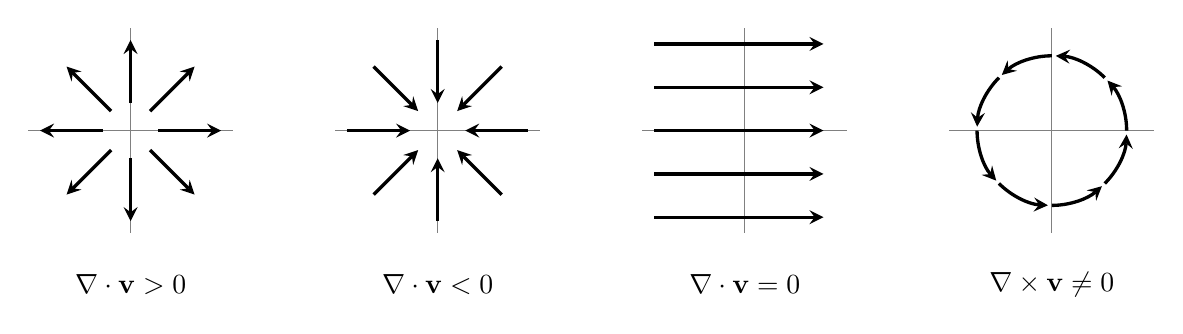
\begin{tikzpicture}[x=0.5cm,y=0.5cm,>=stealth]
 \begin{scope}
  \draw[thin,gray] (-2.6,0) -- (2.6,0); \draw[thin,gray] (0,-2.6) -- (0,2.6);
  \foreach \a in {0,45,...,315}{ \draw[very thick,->] (\a:0.7) -- (\a:2.3); }
  \node at (0,-3.9) {$\nabla\cdot\mathbf{v}>0$};
 \end{scope}
 \begin{scope}[xshift=3.9cm]
  \draw[thin,gray] (-2.6,0) -- (2.6,0); \draw[thin,gray] (0,-2.6) -- (0,2.6);
  \foreach \a in {0,45,...,315}{ \draw[very thick,->] (\a:2.3) -- (\a:0.7); }
  \node at (0,-3.9) {$\nabla\cdot\mathbf{v}<0$};
 \end{scope}
 \begin{scope}[xshift=7.8cm]
  \draw[thin,gray] (-2.6,0) -- (2.6,0); \draw[thin,gray] (0,-2.6) -- (0,2.6);
  \foreach \j in {-2,-1,0,1,2}{ \draw[very thick,->] (-2.3,\j*1.1) -- (2.0,\j*1.1); }
  \node at (0,-3.9) {$\nabla\cdot\mathbf{v}=0$};
 \end{scope}
 \begin{scope}[xshift=11.7cm]
  \draw[thin,gray] (-2.6,0) -- (2.6,0); \draw[thin,gray] (0,-2.6) -- (0,2.6);
  \foreach \a in {0,45,...,315}{ \draw[very thick,->] (\a:1.9) arc[start angle=\a,end angle=\a+42,radius=1.9]; }
  \node at (0,-3.9) {$\nabla\times\mathbf{v}\neq 0$};
 \end{scope}
\end{tikzpicture}
\end{center}

জ্যামিতিক অর্থ ছবির প্রথম তিনটি প্যানেলে। Divergence মাপে ক্ষেত্রটি কোনো
বিন্দু থেকে কতটা \emph{ছড়িয়ে পড়ছে}। ধনাত্মক মানে ওই বিন্দুতে একটি উৎস
(source), ঋণাত্মক মানে একটি ক্ষয়স্থান (sink), শূন্য মানে যতটা ঢুকছে ততটাই
বেরোচ্ছে।

ভৌত পড়া: প্রবাহী পদার্থের বেগ ক্ষেত্রে $\nabla\cdot\mathbf{v}$ বলে দেয়
প্রতি একক আয়তনে কত হারে পদার্থ তৈরি হচ্ছে। অসংনম্য প্রবাহীতে
$\nabla\cdot\mathbf{v} = 0$। তড়িৎচুম্বকত্বে $\nabla\cdot\mathbf{E} =
\rho/\varepsilon_{0}$ (আধানই উৎস) এবং $\nabla\cdot\mathbf{B} = 0$ (চৌম্বক
একক মেরু নেই)।

\begin{example}
$\mathbf{v} = \mathbf{r} = x\hat{\mathbf{x}}+y\hat{\mathbf{y}}
+z\hat{\mathbf{z}}$ এবং $\mathbf{w} = -y\hat{\mathbf{x}}+x\hat{\mathbf{y}}$
এর divergence নির্ণয় করো।
\end{example}

\begin{solbox}
\[
  \nabla\cdot\mathbf{r} = \frac{\partial x}{\partial x}
  + \frac{\partial y}{\partial y} + \frac{\partial z}{\partial z}
  = 1+1+1 = 3 .
\]
\[
  \nabla\cdot\mathbf{w} = \frac{\partial(-y)}{\partial x}
  + \frac{\partial(x)}{\partial y} = 0 + 0 = 0 .
\]
ছবির সঙ্গে মিলিয়ে দেখো: $\mathbf{r}$ সর্বত্র বাইরের দিকে ছড়াচ্ছে, তাই
divergence ধনাত্মক এবং সব বিন্দুতে একই। $\mathbf{w}$ কেবল ঘুরছে, কোথাও
ছড়াচ্ছে না, তাই শূন্য।
\end{solbox}

\prob{3} নিচের প্রতিটির divergence নির্ণয় করো।
\begin{enumerate}
  \item $\mathbf{v} = x^{2}\hat{\mathbf{x}} + 3xz^{2}\hat{\mathbf{y}}
        - 2xz\,\hat{\mathbf{z}}$
  \item $\mathbf{v} = xy\,\hat{\mathbf{x}} + 2yz\,\hat{\mathbf{y}}
        + 3zx\,\hat{\mathbf{z}}$
  \item $\mathbf{v} = \hat{\mathbf{z}}$
\end{enumerate}

\begin{sol}
\begin{enumerate}
  \item $2x + 0 - 2x = 0$।
  \item $y + 2z + 3x$।
  \item সব উপাংশ ধ্রুবক, তাই $0$।
\end{enumerate}
প্রথমটি লক্ষণীয়: ক্ষেত্রটি মোটেই সরল নয়, তবু তার divergence সর্বত্র শূন্য।
\end{sol}

\prob{4} $\mathbf{v} = \dfrac{\hat{\mathbf{r}}}{r^{2}}$ ক্ষেত্রটির জন্য
কার্তেসীয় উপাংশে লিখে দেখাও যে $r \neq 0$-এ $\nabla\cdot\mathbf{v} = 0$।

\begin{sol}
$\hat{\mathbf{r}} = \dfrac{\mathbf{r}}{r}$, তাই
\[
  \mathbf{v} = \frac{\mathbf{r}}{r^{3}}
  = \frac{x\hat{\mathbf{x}}+y\hat{\mathbf{y}}+z\hat{\mathbf{z}}}
  {\left( x^{2}+y^{2}+z^{2} \right)^{3/2}} .
\]
প্রথম উপাংশের derivative নিই। Product ও chain rule (১৫ নম্বর অধ্যায়):
\[
  \frac{\partial}{\partial x}\left( \frac{x}{r^{3}} \right)
  = \frac{1}{r^{3}} + x \cdot \left( -\frac{3}{r^{4}} \right)
    \frac{\partial r}{\partial x} ,
\]
আর $r = \left( x^{2}+y^{2}+z^{2} \right)^{1/2}$ থেকে
$\dfrac{\partial r}{\partial x} = \dfrac{x}{r}$। সুতরাং
\[
  \frac{\partial}{\partial x}\left( \frac{x}{r^{3}} \right)
  = \frac{1}{r^{3}} - \frac{3x^{2}}{r^{5}} .
\]
$y$ ও $z$-এর জন্যও একই আকার। যোগ করি:
\[
  \nabla\cdot\mathbf{v} = \frac{3}{r^{3}}
  - \frac{3\left( x^{2}+y^{2}+z^{2} \right)}{r^{5}}
  = \frac{3}{r^{3}} - \frac{3r^{2}}{r^{5}} = 0 .
\]
মূলবিন্দুতে হিসাবটি অর্থহীন, কারণ সেখানে $r = 0$। এই বাদ পড়া বিন্দুটিই অষ্টম
অনুচ্ছেদের গোটা বিষয়।
\end{sol}

\section{কার্ল}

\begin{idea}[Curl]
\[
  \nabla\times\mathbf{v} =
  \begin{vmatrix}
    \hat{\mathbf{x}} & \hat{\mathbf{y}} & \hat{\mathbf{z}} \\[1mm]
    \dfrac{\partial}{\partial x} & \dfrac{\partial}{\partial y}
    & \dfrac{\partial}{\partial z} \\[1mm]
    v_{x} & v_{y} & v_{z}
  \end{vmatrix} ,
\]
যা একটি vector field। ২০ নম্বর অধ্যায়ের নির্ণায়ক নিয়মে খুললে
\[
  \nabla\times\mathbf{v}
  = \left( \frac{\partial v_{z}}{\partial y}
  - \frac{\partial v_{y}}{\partial z} \right)\hat{\mathbf{x}}
  + \left( \frac{\partial v_{x}}{\partial z}
  - \frac{\partial v_{z}}{\partial x} \right)\hat{\mathbf{y}}
  + \left( \frac{\partial v_{y}}{\partial x}
  - \frac{\partial v_{x}}{\partial y} \right)\hat{\mathbf{z}} .
\]
\end{idea}

জ্যামিতিক অর্থ ছবির শেষ প্যানেলে: curl মাপে ক্ষেত্রটি কোনো বিন্দুর চারপাশে
কতটা \emph{ঘুরছে}। কল্পনা করো ছোট একটি পাখাওয়ালা চাকা প্রবাহে ভাসিয়ে দেওয়া
হলো; সে ঘুরতে শুরু করলে ওই বিন্দুতে curl অশূন্য, আর ঘূর্ণনের অক্ষই curl-এর
দিক।

\begin{idea}[দুটি অভেদ]
\[
  \nabla\times\left( \nabla T \right) = \mathbf{0}, \qquad
  \nabla\cdot\left( \nabla\times\mathbf{v} \right) = 0 .
\]
\end{idea}

দুটিই মিশ্র আংশিক derivative-এর সমতা থেকে আসে (১৫ নম্বর অধ্যায়, যেখানে
$f_{xy} = f_{yx}$ ধরে নেওয়া হয়েছিল)। প্রথমটির $\hat{\mathbf{z}}$ উপাংশ
দেখি:
\[
  \frac{\partial}{\partial x}\left( \frac{\partial T}{\partial y} \right)
  - \frac{\partial}{\partial y}\left( \frac{\partial T}{\partial x} \right)
  = T_{yx} - T_{xy} = 0 .
\]
বাকি উপাংশ ও দ্বিতীয় অভেদটিও হুবহু একইভাবে।

এই দুটি অভেদ পদার্থবিজ্ঞানে অসম্ভব কাজের। ``$\nabla\times\mathbf{E} =
\mathbf{0}$ হলে $\mathbf{E}$-কে কোনো scalar-এর gradient হিসেবে লেখা যায়''
এই কথাটির অর্ধেক এখান থেকেই আসে, আর সেটিই বিভবের ধারণার ভিত্তি।

\begin{example}
$\mathbf{v} = -y\hat{\mathbf{x}} + x\hat{\mathbf{y}}$ এবং
$\mathbf{w} = x\hat{\mathbf{y}}$ এর curl নির্ণয় করো।
\end{example}

\begin{solbox}
প্রথমটির কেবল $\hat{\mathbf{z}}$ উপাংশ টেকে:
\[
  \nabla\times\mathbf{v}
  = \left( \frac{\partial x}{\partial x}
  - \frac{\partial(-y)}{\partial y} \right)\hat{\mathbf{z}}
  = (1+1)\hat{\mathbf{z}} = 2\hat{\mathbf{z}} .
\]
দ্বিতীয়টি:
\[
  \nabla\times\mathbf{w} = \frac{\partial x}{\partial x}\hat{\mathbf{z}}
  = \hat{\mathbf{z}} .
\]
দ্বিতীয়টি চমকপ্রদ। $\mathbf{w}$ ক্ষেত্রে সব তীর $\hat{\mathbf{y}}$ দিকেই,
কোনো ঘূর্ণন চোখে পড়ে না; তবু curl অশূন্য। কারণ ডান দিকে প্রবাহ দ্রুততর, তাই
ভাসানো চাকার ডান পাশের পাখা বাঁ পাশের চেয়ে জোরে ধাক্কা খায় এবং চাকাটি ঘোরে।
Curl মাপে আপেক্ষিক ঘূর্ণন, দেখতে বৃত্তাকার হওয়া জরুরি নয়।
\end{solbox}

\prob{3} নিচের প্রতিটির curl নির্ণয় করো।
\begin{enumerate}
  \item $\mathbf{v} = \mathbf{r}$
  \item $\mathbf{v} = yz\,\hat{\mathbf{x}} + zx\,\hat{\mathbf{y}}
        + xy\,\hat{\mathbf{z}}$
  \item $\mathbf{v} = -y\hat{\mathbf{x}} + x\hat{\mathbf{y}}
        + z\hat{\mathbf{z}}$
\end{enumerate}

\begin{sol}
\begin{enumerate}
  \item প্রতিটি উপাংশ কেবল নিজের চলকের উপর নির্ভর করে, তাই সব আড়াআড়ি
        derivative শূন্য: $\nabla\times\mathbf{r} = \mathbf{0}$।
  \item $\hat{\mathbf{x}}$ উপাংশ: $\dfrac{\partial(xy)}{\partial y}
        - \dfrac{\partial(zx)}{\partial z} = x - x = 0$। বাকি দুটিও একইভাবে
        শূন্য। সুতরাং $\nabla\times\mathbf{v} = \mathbf{0}$।

        (কারণটি লুকিয়ে আছে: $\mathbf{v} = \nabla(xyz)$, আর gradient-এর curl
        সবসময় শূন্য।)
  \item তৃতীয় উপাংশ $z$ যোগ করায় $\hat{\mathbf{z}}$ উপাংশ বদলায় না, তাই
        $\nabla\times\mathbf{v} = 2\hat{\mathbf{z}}$।
\end{enumerate}
\end{sol}

\prob{4} মিশ্র আংশিক derivative-এর সমতা ব্যবহার করে প্রমাণ করো যে
\begin{enumerate}
  \item $\nabla\times(\nabla T) = \mathbf{0}$;
  \item $\nabla\cdot(\nabla\times\mathbf{v}) = 0$।
\end{enumerate}

\begin{sol}
\begin{enumerate}
  \item $\nabla T$-এর উপাংশ $\left( T_{x}, T_{y}, T_{z} \right)$। Curl-এর
        $\hat{\mathbf{x}}$ উপাংশ
        $\dfrac{\partial T_{z}}{\partial y} - \dfrac{\partial T_{y}}
        {\partial z} = T_{zy} - T_{yz} = 0$।
        $\hat{\mathbf{y}}$ ও $\hat{\mathbf{z}}$ উপাংশও একইভাবে শূন্য।
  \item \[
          \nabla\cdot(\nabla\times\mathbf{v})
          = \frac{\partial}{\partial x}\left( \frac{\partial v_{z}}{\partial y}
          - \frac{\partial v_{y}}{\partial z} \right)
          + \frac{\partial}{\partial y}\left( \frac{\partial v_{x}}{\partial z}
          - \frac{\partial v_{z}}{\partial x} \right)
          + \frac{\partial}{\partial z}\left( \frac{\partial v_{y}}{\partial x}
          - \frac{\partial v_{x}}{\partial y} \right) .
        \]
        ছয়টি পদ জোড়ায় জোড়ায় কাটাকাটি যায়:
        $v_{z,yx} - v_{z,xy} = 0$ ইত্যাদি।
\end{enumerate}
দুই ক্ষেত্রেই একমাত্র যা ব্যবহার হলো তা হলো derivative-এর ক্রম বদলানো যায়,
যা ১৫ নম্বর অধ্যায়ে ধরে নেওয়া হয়েছিল।
\end{sol}

\section{ল্যাপ্লাসিয়ান}

\begin{idea}[Laplacian]
\[
  \nabla^{2}T = \nabla\cdot(\nabla T)
  = \frac{\partial^{2}T}{\partial x^{2}}
  + \frac{\partial^{2}T}{\partial y^{2}}
  + \frac{\partial^{2}T}{\partial z^{2}} .
\]
ভেক্টরের ক্ষেত্রে $\nabla^{2}\mathbf{v}$ মানে প্রতিটি উপাংশে আলাদা করে একই
কাজ।
\end{idea}

$\nabla$-এর পাঁচটি সম্ভাব্য দ্বিতীয় স্তরের সমন্বয়ের মধ্যে এটিই সবচেয়ে
বেশি লাগে, কারণ পদার্থবিজ্ঞানের প্রায় প্রতিটি মৌলিক সমীকরণে সে আছে:
\[
  \nabla^{2}V = -\frac{\rho}{\varepsilon_{0}}, \qquad
  \nabla^{2}T = \frac{1}{\alpha}\frac{\partial T}{\partial t}, \qquad
  \nabla^{2}\mathbf{E} = \frac{1}{c^{2}}
  \frac{\partial^{2}\mathbf{E}}{\partial t^{2}} .
\]
এগুলো যথাক্রমে Poisson-এর সমীকরণ, তাপ সমীকরণ ও তরঙ্গ সমীকরণ। ১৯ নম্বর
অধ্যায়ে বলা হয়েছিল যে এরা PDE এবং এই সিরিজে সমাধান করা হবে না; এখানে
কেবল লেখার ভাষাটুকু তৈরি হলো।

\begin{idea}[অর্থ]
$\nabla^{2}T$ মাপে কোনো বিন্দুতে $T$-এর মান তার চারপাশের গড় থেকে কতটা কম।
$\nabla^{2}T > 0$ মানে বিন্দুটি প্রতিবেশীদের গড়ের চেয়ে নিচু (গর্তের তলা),
$< 0$ মানে উঁচু (ঢিবির চূড়া), আর $= 0$ মানে ঠিক গড়ের সমান।
\end{idea}

এই ``গড়'' বিবৃতিটি একটি উপপাদ্য এবং এখানে প্রমাণ করা হচ্ছে না; ধরে নেওয়া
হচ্ছে। তবে এক মাত্রায় ইন্টুইশনটা পরিষ্কার: $T'' > 0$ মানে বক্ররেখা উপরের দিকে
বাঁকা (১৫ নম্বর অধ্যায়ের concavity), অর্থাৎ দুই পাশের মানের গড় মাঝের
মানের চেয়ে বেশি।

$\nabla^{2}T = 0$ হলে $T$-কে বলে harmonic। উপরের অর্থ থেকেই একটি চমৎকার ফল
আসে: harmonic ফাংশনের কোনো অভ্যন্তরীণ চরম মান থাকতে পারে না, কারণ চূড়া হতে
হলে তাকে প্রতিবেশীদের গড়ের চেয়ে উঁচু হতে হতো।

\begin{example}
$T = \dfrac{1}{r}$ ($r \neq 0$) harmonic কি না যাচাই করো।
\end{example}

\begin{solbox}
কার্তেসীয়ভাবে করা যায়, কিন্তু নবম অনুচ্ছেদের spherical সূত্রে অনেক সহজ। ওই
সূত্রে ($T$ কেবল $r$-এর উপর নির্ভর করলে)
\[
  \nabla^{2}T = \frac{1}{r^{2}}\frac{d}{dr}
  \left( r^{2}\frac{dT}{dr} \right) .
\]
এখানে $\dfrac{dT}{dr} = -\dfrac{1}{r^{2}}$, তাই
$r^{2}\dfrac{dT}{dr} = -1$, একটি ধ্রুবক। ধ্রুবকের derivative শূন্য, সুতরাং
\[
  \nabla^{2}\left( \frac{1}{r} \right) = 0 \qquad (r \neq 0) .
\]
অর্থাৎ $1/r$ সর্বত্র harmonic, মূলবিন্দু বাদে। আর মূলবিন্দুতে কী হয়, সেটিই
অষ্টম অনুচ্ছেদের প্রশ্ন। ভৌতভাবে $1/r$ হলো বিন্দু আধানের বিভব, আর
Poisson-এর সমীকরণ বলছে আধান যেখানে নেই সেখানে $\nabla^{2}V = 0$; মিলে যাচ্ছে।
\end{solbox}

\prob{3} নিচের প্রতিটির Laplacian নির্ণয় করো।
\begin{enumerate}
  \item $T = x^{2}+y^{2}+z^{2}$
  \item $T = x^{2}-y^{2}$
  \item $T = e^{x}\sin y$
\end{enumerate}

\begin{sol}
\begin{enumerate}
  \item $2+2+2 = 6$।
  \item $2 + (-2) = 0$, অর্থাৎ harmonic।
  \item $e^{x}\sin y + e^{x}(-\sin y) = 0$, আবার harmonic।
\end{enumerate}
\end{sol}

\prob{4} $T = x^{2}-y^{2}$ ক্ষেত্রটি বিবেচনা করো।
\begin{enumerate}
  \item দেখাও যে $(0,0)$ একটি critical point ($\nabla T = \mathbf{0}$)।
  \item দেখাও যে সেখানে $T$-এর স্থানীয় সর্বোচ্চও নেই, সর্বনিম্নও নেই।
  \item ব্যাখ্যা করো কেন $\nabla^{2}T = 0$ থাকলে অভ্যন্তরীণ চরম মান থাকতে
        পারে না।
\end{enumerate}

\begin{sol}
\begin{enumerate}
  \item $\nabla T = 2x\hat{\mathbf{x}} - 2y\hat{\mathbf{y}}$, যা $(0,0)$-এ
        শূন্য।
  \item $x$-অক্ষ বরাবর ($y=0$) $T = x^{2} > 0$, অর্থাৎ মূলবিন্দুর চেয়ে বড়।
        $y$-অক্ষ বরাবর ($x=0$) $T = -y^{2} < 0$, অর্থাৎ ছোট। এক দিকে বাড়ে,
        অন্য দিকে কমে, তাই এটি saddle point।
  \item স্থানীয় সর্বোচ্চ হতে হলে সব দিকেই দ্বিতীয় derivative অঋণাত্মক নয়,
        বরং অ-ধনাত্মক হতে হতো, অর্থাৎ $T_{xx} \leq 0$, $T_{yy} \leq 0$ এবং
        $T_{zz} \leq 0$। তখন তাদের যোগফলও অ-ধনাত্মক, আর $\nabla^{2}T = 0$
        হলে তিনটিকেই শূন্য হতে হতো, যা কড়া চরম মানের সঙ্গে খাপ খায় না।

        আরও সরল পাঠ: $\nabla^{2}T = 0$ মানে প্রতিটি বিন্দুর মান তার
        প্রতিবেশীদের গড়ের সমান; কিন্তু চূড়ায় মান গড়ের চেয়ে বেশি হতে বাধ্য।
\end{enumerate}
\end{sol}

\section{রেখা, তল ও আয়তন ইন্টিগ্রাল}

১৭ নম্বর অধ্যায়ে ইন্টিগ্রাল ছিল একটি ব্যবধির উপর। এখন পথ, তল ও আয়তনের
উপর একই কাজ করব, আর উপাদানগুলো ১৬ নম্বর অধ্যায়ে তৈরি হয়ে আছে।

\begin{idea}[তিন ধরনের ইন্টিগ্রাল]
\[
  \int_{a}^{b} \mathbf{v}\cdot d\mathbf{l}
  \quad (\text{পথ বরাবর}), \qquad
  \int_{S} \mathbf{v}\cdot d\mathbf{a}
  \quad (\text{তলের উপর}), \qquad
  \int_{V} T \, d\tau
  \quad (\text{আয়তনের উপর}) .
\]
এখানে $d\mathbf{l}$ পথের স্পর্শক বরাবর ক্ষুদ্র সরণ, $d\mathbf{a} =
\hat{\mathbf{n}}\,da$ তলের অভিলম্ব বরাবর ক্ষুদ্র ক্ষেত্রফল, আর $d\tau$
ক্ষুদ্র আয়তন। বদ্ধ পথ ও বদ্ধ তলের জন্য লেখা হয়
$\oint \mathbf{v}\cdot d\mathbf{l}$ ও
$\oint_{S}\mathbf{v}\cdot d\mathbf{a}$।
\end{idea}

দ্বিতীয়টির নাম flux, এবং সেটি ১৬ নম্বর অধ্যায়ে ইঙ্গিত করা রাশিটিই। ভৌত
অর্থ: প্রতি একক সময়ে তলটি দিয়ে কতটা ``পার হচ্ছে''। $\hat{\mathbf{n}}$ কোন
দিকে ধরা হলো তার উপর চিহ্ন নির্ভর করে, তাই বদ্ধ তলের ক্ষেত্রে সবসময় বাইরের
দিকে ধরা হয়।

প্রথমটির নাম circulation বা কৃতকাজ। $\mathbf{v} = \mathbf{F}$ হলে
$\int\mathbf{F}\cdot d\mathbf{l}$ হলো কাজ, যা ১৭ নম্বর অধ্যায়ের
$\int F\,dx$-এর ত্রিমাত্রিক সাধারণ রূপ।

\begin{remark}
একটি সতর্কতা যা পদার্থবিজ্ঞানে খুব গুরুত্বপূর্ণ: রেখা-ইন্টিগ্রালের মান
সাধারণত \emph{পথের উপর নির্ভর করে}, কেবল দুই প্রান্তবিন্দুর উপর নয়। যেসব
ক্ষেত্রে নির্ভর করে না, তাদের বলে conservative, আর সপ্তম অনুচ্ছেদে দেখা যাবে
যে সেটি ঘটে ঠিক তখনই যখন ক্ষেত্রটি কোনো scalar-এর gradient। মহাকর্ষ ও
স্থির তড়িৎ ক্ষেত্র conservative; ঘর্ষণ নয়।
\end{remark}

\begin{example}
$\mathbf{v} = y\hat{\mathbf{x}} + 2x\hat{\mathbf{y}}$ ক্ষেত্রে $(0,0)$ থেকে
$(1,1)$ পর্যন্ত $\int\mathbf{v}\cdot d\mathbf{l}$ নির্ণয় করো
(ক) সরলরেখা বরাবর, (খ) আগে $x$-অক্ষ ধরে $(1,0)$, তারপর উপরে $(1,1)$।
\end{example}

\begin{solbox}
সাধারণভাবে $\mathbf{v}\cdot d\mathbf{l} = y\,dx + 2x\,dy$।

(ক) সরলরেখায় $y = x$, তাই $dy = dx$ এবং
\[
  \int_{0}^{1}\left( x\,dx + 2x\,dx \right) = \int_{0}^{1}3x\,dx
  = \frac{3}{2} .
\]

(খ) প্রথম টুকরোয় $y = 0$ ও $dy = 0$, তাই অবদান শূন্য। দ্বিতীয় টুকরোয়
$x = 1$ ও $dx = 0$, তাই
\[
  \int_{0}^{1}2\,dy = 2 .
\]
মোট $2$।

দুটি আলাদা, তাই এই ক্ষেত্রটি conservative নয়। যাচাই:
$\nabla\times\mathbf{v} = \left( \dfrac{\partial(2x)}{\partial x}
- \dfrac{\partial y}{\partial y} \right)\hat{\mathbf{z}}
= (2-1)\hat{\mathbf{z}} = \hat{\mathbf{z}} \neq \mathbf{0}$।
\end{solbox}

\prob{3} $\mathbf{v} = x^{2}\hat{\mathbf{x}} + xy\,\hat{\mathbf{y}}$
ক্ষেত্রে $(0,0)$ থেকে $(1,1)$ পর্যন্ত $\int\mathbf{v}\cdot d\mathbf{l}$
নির্ণয় করো (ক) $y = x$ বরাবর, (খ) $y = x^{2}$ বরাবর। ক্ষেত্রটি
conservative কি না বলো।

\begin{sol}
$\mathbf{v}\cdot d\mathbf{l} = x^{2}dx + xy\,dy$।

(ক) $y = x$, $dy = dx$:
\[
  \int_{0}^{1}\left( x^{2} + x^{2} \right)dx = \frac{2}{3} .
\]

(খ) $y = x^{2}$, $dy = 2x\,dx$:
\[
  \int_{0}^{1}\left( x^{2} + x\cdot x^{2}\cdot 2x \right)dx
  = \int_{0}^{1}\left( x^{2} + 2x^{4} \right)dx
  = \frac{1}{3} + \frac{2}{5} = \frac{11}{15} .
\]
$\dfrac{2}{3} = \dfrac{10}{15} \neq \dfrac{11}{15}$, তাই পথের উপর নির্ভর
করছে; ক্ষেত্রটি conservative নয়।

যাচাই: $\nabla\times\mathbf{v} = \left( \dfrac{\partial(xy)}{\partial x}
- \dfrac{\partial(x^{2})}{\partial y} \right)\hat{\mathbf{z}}
= y\,\hat{\mathbf{z}} \neq \mathbf{0}$।
\end{sol}

\prob{4} $R$ ব্যাসার্ধের একটি গোলকের পৃষ্ঠ দিয়ে
$\mathbf{v} = \mathbf{r}$ ক্ষেত্রের flux নির্ণয় করো, সরাসরি হিসাব করে।
এরপর $\nabla\cdot\mathbf{v}$ ব্যবহার করে ফলটি যাচাই করো।

\begin{sol}
গোলকের পৃষ্ঠে $\mathbf{r} = R\hat{\mathbf{r}}$ এবং বাইরের অভিলম্ব
$\hat{\mathbf{n}} = \hat{\mathbf{r}}$, তাই
\[
  \mathbf{v}\cdot d\mathbf{a} = R\,da .
\]
১৬ নম্বর অধ্যায় থেকে $da = R^{2}\sin\theta\,d\theta\,d\phi$, সুতরাং
\[
  \oint\mathbf{v}\cdot d\mathbf{a}
  = R^{3}\int_{0}^{\pi}\sin\theta\,d\theta\int_{0}^{2\pi}d\phi
  = R^{3}\cdot 2 \cdot 2\pi = 4\pi R^{3} .
\]
(অথবা আরও সংক্ষেপে: $R$ ধ্রুবক, তাই flux $= R \times$ মোট পৃষ্ঠতল
$= R\cdot 4\pi R^{2}$।)

যাচাই: $\nabla\cdot\mathbf{r} = 3$, আর গোলকের আয়তন $\tfrac{4}{3}\pi R^{3}$
(১১ ও ১৭ নম্বর অধ্যায়), তাই
\[
  \int_{V}(\nabla\cdot\mathbf{v})\,d\tau = 3 \cdot \frac{4}{3}\pi R^{3}
  = 4\pi R^{3} .
\]
দুটি মিলে গেল; পরের অনুচ্ছেদ বলবে কেন এটি কাকতালীয় নয়।
\end{sol}

\section{মৌলিক উপপাদ্যসমূহ}

তিনটি উপপাদ্য, একটিই কাঠামো।

\begin{idea}[Gradient theorem]
\[
  \int_{\mathbf{a}}^{\mathbf{b}} \left( \nabla T \right)\cdot d\mathbf{l}
  = T(\mathbf{b}) - T(\mathbf{a}) ,
\]
পথ যাই হোক। ফলে $\oint\left( \nabla T \right)\cdot d\mathbf{l} = 0$।
\end{idea}

\begin{idea}[Divergence theorem, Gauss]
\[
  \int_{V}\left( \nabla\cdot\mathbf{v} \right)d\tau
  = \oint_{S}\mathbf{v}\cdot d\mathbf{a} ,
\]
যেখানে $S$ হলো $V$-এর সীমানা।
\end{idea}

\begin{idea}[Stokes theorem]
\[
  \int_{S}\left( \nabla\times\mathbf{v} \right)\cdot d\mathbf{a}
  = \oint_{P}\mathbf{v}\cdot d\mathbf{l} ,
\]
যেখানে $P$ হলো $S$-এর সীমানা-রেখা।
\end{idea}

তিনটিরই প্রমাণ এখানে দেওয়া হচ্ছে না; ধরে নেওয়া হচ্ছে। কিন্তু কাঠামোটা
চোখে পড়া দরকার, কারণ সেটিই আসল শিক্ষা।

প্রতিটি বলছে: \emph{ভেতরে $\nabla$-এর কোনো এক রূপের যোগফল সমান সীমানার উপর
মূল রাশিটির যোগফল}। Gradient theorem-এ ভেতরটা একটি রেখা আর সীমানা দুটি
বিন্দু; divergence theorem-এ ভেতরটা একটি আয়তন আর সীমানা একটি বদ্ধ তল;
Stokes-এ ভেতরটা একটি তল আর সীমানা একটি বদ্ধ রেখা।

আর ১৭ নম্বর অধ্যায়ের মৌলিক উপপাদ্যও একই কথা বলত:
$\int_{a}^{b}f'\,dx = f(b)-f(a)$, যেখানে ভেতরটা একটি ব্যবধি আর সীমানা তার
দুই প্রান্ত। চারটিই একই উপপাদ্যের চার মাত্রার রূপ।

Gradient theorem-এর একটি সরাসরি ফল ষষ্ঠ অনুচ্ছেদের প্রশ্নের উত্তর দেয়:
$\mathbf{v} = \nabla T$ হলে রেখা-ইন্টিগ্রাল কেবল দুই প্রান্তের উপর নির্ভর
করে, অর্থাৎ ক্ষেত্রটি conservative। আর চতুর্থ অনুচ্ছেদের অভেদ অনুযায়ী তখন
$\nabla\times\mathbf{v} = \mathbf{0}$।

\begin{example}
$a$ বাহুর একটি ঘনকের জন্য (এক কোণ মূলবিন্দুতে, ধারগুলো অক্ষ বরাবর)
$\mathbf{v} = \mathbf{r}$ ক্ষেত্রে divergence theorem যাচাই করো।
\end{example}

\begin{solbox}
বাম পাশ: $\nabla\cdot\mathbf{r} = 3$, তাই
\[
  \int_{V}3\,d\tau = 3a^{3} .
\]

ডান পাশ: ছয়টি তল। মূলবিন্দুর দিকের তিনটি তলে (যেমন $x=0$ তল) বাইরের অভিলম্ব
$-\hat{\mathbf{x}}$, আর ওই তলে $\mathbf{r}$-এর $x$ উপাংশ শূন্য; তাই অবদান
শূন্য। বাকি তিনটি তলের একটি ধরি, $x = a$: সেখানে
$\hat{\mathbf{n}} = \hat{\mathbf{x}}$ এবং
$\mathbf{r}\cdot\hat{\mathbf{n}} = a$, তাই অবদান $a \cdot a^{2} = a^{3}$।
তিনটি মিলে $3a^{3}$।

দুই পাশ সমান। খেয়াল করো, বাম পাশে একটিমাত্র সহজ ইন্টিগ্রাল আর ডান পাশে ছয়টি
আলাদা হিসাব লাগল; উপপাদ্যটির ব্যবহারিক মূল্য ঠিক এখানেই।
\end{solbox}

\prob{4} $\mathbf{v} = -y\hat{\mathbf{x}} + x\hat{\mathbf{y}}$ ক্ষেত্রে
$z=0$ সমতলে $R$ ব্যাসার্ধের চাকতির জন্য Stokes-এর উপপাদ্য যাচাই করো।

\begin{sol}
বাম পাশ: চতুর্থ অনুচ্ছেদ থেকে $\nabla\times\mathbf{v} = 2\hat{\mathbf{z}}$।
চাকতির অভিলম্ব $\hat{\mathbf{z}}$, তাই
\[
  \int_{S}\left( \nabla\times\mathbf{v} \right)\cdot d\mathbf{a}
  = 2 \times (\text{চাকতির ক্ষেত্রফল}) = 2\pi R^{2} .
\]

ডান পাশ: সীমানা-বৃত্তে $x = R\cos t$, $y = R\sin t$, তাই
$dx = -R\sin t\,dt$ এবং $dy = R\cos t\,dt$। এখন
\[
  \mathbf{v}\cdot d\mathbf{l} = -y\,dx + x\,dy
  = R^{2}\sin^{2}t\,dt + R^{2}\cos^{2}t\,dt = R^{2}dt .
\]
$t$-কে $0$ থেকে $2\pi$ চালিয়ে
\[
  \oint\mathbf{v}\cdot d\mathbf{l} = 2\pi R^{2} .
\]
দুই পাশ সমান।
\end{sol}

\prob{4} $\mathbf{v} = \nabla T$ হলে প্রমাণ করো যে
\begin{enumerate}
  \item $\int\mathbf{v}\cdot d\mathbf{l}$ পথের উপর নির্ভর করে না;
  \item $\nabla\times\mathbf{v} = \mathbf{0}$;
  \item $\mathbf{v} = y\hat{\mathbf{x}} + 2x\hat{\mathbf{y}}$ কোনো
        scalar-এর gradient হতে পারে না।
\end{enumerate}

\begin{sol}
\begin{enumerate}
  \item Gradient theorem অনুযায়ী ইন্টিগ্রালটি $T(\mathbf{b}) -
        T(\mathbf{a})$, যেখানে পথের কোনো উল্লেখ নেই।
  \item চতুর্থ অনুচ্ছেদের অভেদ: $\nabla\times(\nabla T) = \mathbf{0}$।
  \item ষষ্ঠ অনুচ্ছেদের উদাহরণে দেখা গেছে
        $\nabla\times\mathbf{v} = \hat{\mathbf{z}} \neq \mathbf{0}$।
        (২) অনুযায়ী gradient হলে curl শূন্য হতেই হতো, তাই এটি কোনো
        scalar-এর gradient নয়। একই কথা রেখা-ইন্টিগ্রাল থেকেও বলা যায়:
        দুটি পথে দুটি আলাদা উত্তর এসেছিল।
\end{enumerate}
\end{sol}

\prob{5} বিন্দু আধান $q$-এর ক্ষেত্র
$\mathbf{E} = \dfrac{q}{4\pi\varepsilon_{0}}\dfrac{\hat{\mathbf{r}}}{r^{2}}$।
\begin{enumerate}
  \item দেখাও যে আধানকে ঘিরে থাকা \emph{যেকোনো} বদ্ধ তলের ভেতর দিয়ে flux
        $\dfrac{q}{\varepsilon_{0}}$, তলটির আকার যাই হোক। (ইঙ্গিত: ১১ নম্বর
        অধ্যায়ের solid angle ব্যবহার করো।)
  \item আধান তলের বাইরে থাকলে flux কত, এবং কেন?
\end{enumerate}

\begin{sol}
\begin{enumerate}
  \item তলের একটি ক্ষুদ্র টুকরো $d\mathbf{a}$ নাও, যা আধান থেকে $r$ দূরে এবং
        যার অভিলম্ব ব্যাসার্ধের সঙ্গে $\alpha$ কোণ করে। তখন
        \[
          \mathbf{E}\cdot d\mathbf{a}
          = \frac{q}{4\pi\varepsilon_{0}}\frac{da\cos\alpha}{r^{2}} .
        \]
        কিন্তু $da\cos\alpha$ হলো টুকরোটির ব্যাসার্ধের লম্বদিকে অভিক্ষিপ্ত
        ক্ষেত্রফল, তাই ১১ নম্বর অধ্যায়ের সংজ্ঞা অনুযায়ী
        $\dfrac{da\cos\alpha}{r^{2}} = d\Omega$, ওই টুকরোটি আধান থেকে যে
        solid angle জুড়ে আছে। সুতরাং
        \[
          \oint\mathbf{E}\cdot d\mathbf{a}
          = \frac{q}{4\pi\varepsilon_{0}}\oint d\Omega
          = \frac{q}{4\pi\varepsilon_{0}} \cdot 4\pi
          = \frac{q}{\varepsilon_{0}} ,
        \]
        যেখানে ১১ নম্বর অধ্যায়ের ফল ব্যবহার করা হলো যে একটি বিন্দুর
        চারপাশে মোট solid angle $4\pi$।

        লক্ষ করো, $r$ কোথাও টেকেনি; তাই তলের আকার ও দূরত্ব কিছুই যায় আসে না।
  \item শূন্য। আধান বাইরে থাকলে তার থেকে বেরোনো যেকোনো সরু cone তলটিকে জোড়ায়
        জোড়ায় কাটে: একবার ঢোকার সময়, একবার বেরোনোর সময়। দুটি টুকরোর
        solid angle সমান কিন্তু $\cos\alpha$-এর চিহ্ন উল্টো, তাই অবদান
        দুটি কাটাকাটি যায়। সব cone-এর জন্য একই কথা, তাই মোট flux শূন্য।
\end{enumerate}
এটিই Gauss-এর সূত্র। ১১ নম্বর অধ্যায়ে যে ইঙ্গিত দেওয়া হয়েছিল, সেটি
এখানে পূর্ণ হলো: solid angle-ই এই সূত্রের আসল ইঞ্জিন, আর
$\dfrac{1}{r^{2}}$ ও $r^{2}\,d\Omega$ ঠিক ঠিক কাটাকাটি যায় বলেই ফলটি এত
সরল।
\end{sol}

\section{ডিরাক ডেল্টা}

এখন একটি স্ববিরোধ, এবং তার সমাধান।

তৃতীয় অনুচ্ছেদের সমস্যায় দেখা গেছে $\nabla\cdot\left(
\dfrac{\hat{\mathbf{r}}}{r^{2}} \right) = 0$ সব $r \neq 0$-এ। তাহলে
divergence theorem অনুযায়ী মূলবিন্দু ঘিরে থাকা যেকোনো গোলকের flux শূন্য
হওয়া উচিত। অথচ সরাসরি হিসাব করলে
\[
  \oint \frac{\hat{\mathbf{r}}}{r^{2}}\cdot d\mathbf{a}
  = \int \frac{1}{R^{2}} R^{2}\sin\theta\,d\theta\,d\phi = 4\pi ,
\]
শূন্য নয়। কোথাও একটা গোলমাল।

গোলমালটা মূলবিন্দুতে। সেখানে ক্ষেত্রটি অসীম, আর divergence-এর হিসাবটি
অর্থহীন। সব ``ছড়ানো'' ওই একটিমাত্র বিন্দুতে জমা হয়ে আছে।

\begin{idea}[এক মাত্রায় ডেল্টা]
$\delta(x)$ এমন একটি বস্তু যার জন্য
\[
  \delta(x) = 0 \quad (x \neq 0), \qquad
  \int_{-\infty}^{\infty}\delta(x)\,dx = 1 .
\]
এর প্রধান ধর্ম (sifting property):
\[
  \int_{-\infty}^{\infty} f(x)\,\delta(x-a)\,dx = f(a) .
\]
\end{idea}

\begin{center}
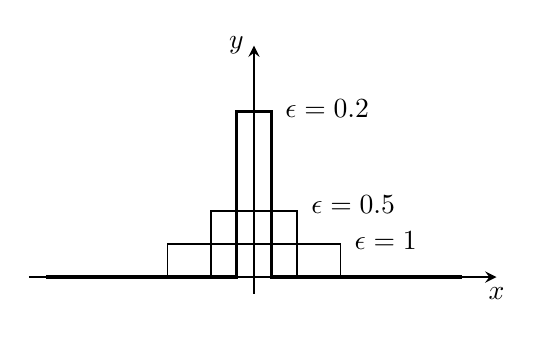
\begin{tikzpicture}[x=1.1cm,y=0.42cm,>=stealth]
  \draw[thick,->] (-2.6,0) -- (2.8,0) node[below] {$x$};
  \draw[thick,->] (0,-0.5) -- (0,7.0) node[left] {$y$};
  \draw[thin] (-2.4,0) -- (-1.0,0) -- (-1.0,1) -- (1.0,1) -- (1.0,0) -- (2.4,0);
  \draw[thick] (-2.4,0) -- (-0.5,0) -- (-0.5,2) -- (0.5,2) -- (0.5,0) -- (2.4,0);
  \draw[very thick] (-2.4,0) -- (-0.2,0) -- (-0.2,5) -- (0.2,5) -- (0.2,0) -- (2.4,0);
  \node[right] at (1.05,1.1) {$\epsilon=1$};
  \node[right] at (0.55,2.2) {$\epsilon=0.5$};
  \node[right] at (0.25,5.1) {$\epsilon=0.2$};
\end{tikzpicture}
\end{center}

\begin{remark}
এখানে খুব স্পষ্ট করে বলা দরকার: \emph{$\delta$ কোনো ফাংশন নয়}। কোনো
সত্যিকারের ফাংশন একটিমাত্র বিন্দু ছাড়া সর্বত্র শূন্য হয়ে এক ইউনিট
ক্ষেত্রফল রাখতে পারে না; ১৭ নম্বর অধ্যায়ের Riemann sum-এ সেটি সবসময়
শূন্য দিত।

সঠিক পাঠ ছবিটিই: $\delta$ হলো ক্রমশ সরু ও উঁচু শিখরের একটি \emph{সীমা}।
ছবিতে প্রতিটি আয়তক্ষেত্রের প্রস্থ $\epsilon$ ও উচ্চতা $1/\epsilon$, তাই
ক্ষেত্রফল সবসময় $1$; $\epsilon \to 0$ নিলে যা পাওয়া যায় তাকেই $\delta$ বলা
হয়। কড়া গণিতে এই বস্তুটির নাম distribution, এবং তার তত্ত্ব এই সিরিজের
বাইরে; আমরা কেবল উপরের দুটি ধর্ম ধরে নিয়ে কাজ চালাব।

ব্যবহারিক নিয়ম: $\delta$ একা দাঁড়িয়ে কিছু বোঝায় না, সে কেবল
ইন্টিগ্রালের ভেতরে অর্থবহ।
\end{remark}

Sifting property-র কারণ সহজ: $\delta(x-a)$ কেবল $x = a$-এর কাছেই অশূন্য, আর
ওই ক্ষুদ্র এলাকায় $f$ প্রায় ধ্রুবক $f(a)$; তাই $f(a)$ বাইরে বেরিয়ে আসে এবং
বাকি থাকে $\int\delta = 1$।

\begin{idea}[তিন মাত্রায়]
\[
  \delta^{3}(\mathbf{r}) = \delta(x)\delta(y)\delta(z), \qquad
  \int_{\text{সমগ্র স্থান}} \delta^{3}(\mathbf{r})\,d\tau = 1 ,
\]
এবং উপরের স্ববিরোধের সমাধান:
\[
  \nabla\cdot\left( \frac{\hat{\mathbf{r}}}{r^{2}} \right)
  = 4\pi\,\delta^{3}(\mathbf{r}) .
\]
\end{idea}

এটিই দুই দিককে মিলিয়ে দেয়। $r \neq 0$-এ ডান পাশ শূন্য, যা তৃতীয় অনুচ্ছেদের
হিসাবের সঙ্গে মেলে। আর যেকোনো আয়তনে integrate করলে, যদি মূলবিন্দু ভেতরে
থাকে, $4\pi\int\delta^{3}\,d\tau = 4\pi$ পাওয়া যায়, যা flux-এর সঙ্গে মেলে।

ভৌত ভাষায়: বিন্দু আধানের আধান-ঘনত্ব সর্বত্র শূন্য অথচ মোট আধান $q$; একে
লিখতে হলে $\rho = q\,\delta^{3}(\mathbf{r})$ ছাড়া উপায় নেই। Gauss-এর সূত্রের
অন্তরক রূপ $\nabla\cdot\mathbf{E} = \rho/\varepsilon_{0}$ তখন ঠিক ঠিক
কাজ করে।

\begin{example}
নির্ণয় করো: (ক) $\int_{-\infty}^{\infty}\left( x^{2}+3 \right)
\delta(x-2)\,dx$; (খ) $\int_{0}^{5} x\,\delta(x-7)\,dx$।
\end{example}

\begin{solbox}
(ক) Sifting property সরাসরি: মান হলো $x = 2$-তে integrand-এর বাকি অংশ,
অর্থাৎ $4 + 3 = 7$।

(খ) শিখরটি $x = 7$-এ, যা $[0,5]$ ব্যবধির বাইরে। ওই ব্যবধিতে $\delta(x-7)$
সর্বত্র শূন্য, তাই ইন্টিগ্রাল $0$।

দ্বিতীয়টি মনে রাখার মতো: $\delta$ কেবল তখনই কিছু দেয়, যখন তার শিখরটি
সমাকলনের সীমার ভেতরে পড়ে।
\end{solbox}

\prob{4} নির্ণয় করো।
\begin{enumerate}
  \item $\int_{-\infty}^{\infty}\left( 3x^{2} - 2x + 1 \right)\delta(x-3)\,dx$
  \item $\int_{-1}^{4} e^{-x}\,\delta(x-2)\,dx$
  \item $\int_{-\infty}^{\infty} \cos x\,\delta(x)\,dx$
\end{enumerate}

\begin{sol}
\begin{enumerate}
  \item $x = 3$ বসিয়ে $27 - 6 + 1 = 22$।
  \item শিখর $x=2$ ব্যবধির ভেতরে, তাই $e^{-2} \approx 0.135$।
  \item $x = 0$ বসিয়ে $\cos 0 = 1$।
\end{enumerate}
\end{sol}

\prob{5} তৃতীয় অনুচ্ছেদে পাওয়া গিয়েছিল $\nabla\cdot\left(
\hat{\mathbf{r}}/r^{2} \right) = 0$ ($r\neq 0$), অথচ ষষ্ঠ অনুচ্ছেদের কায়দায়
হিসাব করলে যেকোনো গোলকের flux $4\pi$।
\begin{enumerate}
  \item flux-টি সরাসরি হিসাব করে দেখাও যে সত্যিই $4\pi$, এবং লক্ষ করো যে
        উত্তরে $R$ নেই।
  \item ব্যাখ্যা করো কেন এতে divergence theorem ভাঙে না।
  \item $\nabla\cdot\left( \hat{\mathbf{r}}/r^{2} \right)
        = 4\pi\delta^{3}(\mathbf{r})$ ধরে নিয়ে দেখাও যে উপপাদ্যের দুই পাশ
        মিলে যায়।
\end{enumerate}

\begin{sol}
\begin{enumerate}
  \item $R$ ব্যাসার্ধের গোলকে $\hat{\mathbf{n}} = \hat{\mathbf{r}}$ এবং
        ক্ষেত্রের মান $1/R^{2}$, তাই
        \[
          \oint\frac{\hat{\mathbf{r}}}{r^{2}}\cdot d\mathbf{a}
          = \frac{1}{R^{2}} \times 4\pi R^{2} = 4\pi .
        \]
        $R$ কাটাকাটি গেছে, তাই ফল ব্যাসার্ধ-নিরপেক্ষ।
  \item Divergence theorem প্রয়োগ করতে হলে ক্ষেত্র ও তার derivative-কে
        গোটা আয়তনে ভদ্র হতে হয়। এখানে মূলবিন্দুতে ক্ষেত্রটি অসীম, তাই
        সেখানে ``$\nabla\cdot\mathbf{v} = 0$'' বলাই অর্থহীন; হিসাবটি কেবল
        $r\neq 0$-এ বৈধ ছিল। ভাঙা পড়েছে অনুমান, উপপাদ্য নয়।
  \item ধরে নেওয়া রূপটি বসাই:
        \[
          \int_{V}\nabla\cdot\left( \frac{\hat{\mathbf{r}}}{r^{2}} \right)
          d\tau = \int_{V}4\pi\delta^{3}(\mathbf{r})\,d\tau = 4\pi ,
        \]
        কারণ মূলবিন্দু $V$-এর ভেতরে। এটি ঠিক flux-এর সমান, তাই দুই পাশ
        মিলে গেল।

        আর মূলবিন্দু যদি $V$-এর বাইরে থাকত, তবে integral শূন্য হতো, আর
        সপ্তম অনুচ্ছেদের শেষ সমস্যা অনুযায়ী flux-ও শূন্য। দুই ক্ষেত্রেই
        সংগতিপূর্ণ।
\end{enumerate}
\end{sol}

\section{বক্ররৈখিক স্থানাঙ্কে}

শেষ অনুচ্ছেদ। ১২ নম্বর অধ্যায়ে cylindrical $(s,\phi,z)$ ও spherical
$(r,\theta,\phi)$ স্থানাঙ্ক তৈরি হয়েছিল এবং ১৬ নম্বরে তাদের ক্ষুদ্র উপাদান।
এবার $\nabla$-এর রূপগুলো।

\begin{idea}[Spherical স্থানাঙ্কে]
\[
  d\mathbf{l} = dr\,\hat{\mathbf{r}} + r\,d\theta\,\hat{\boldsymbol{\theta}}
  + r\sin\theta\,d\phi\,\hat{\boldsymbol{\phi}}, \qquad
  d\tau = r^{2}\sin\theta\,dr\,d\theta\,d\phi ,
\]
\[
  \nabla T = \frac{\partial T}{\partial r}\hat{\mathbf{r}}
  + \frac{1}{r}\frac{\partial T}{\partial\theta}\hat{\boldsymbol{\theta}}
  + \frac{1}{r\sin\theta}\frac{\partial T}{\partial\phi}
  \hat{\boldsymbol{\phi}} ,
\]
\[
  \nabla\cdot\mathbf{v} = \frac{1}{r^{2}}
  \frac{\partial\left( r^{2}v_{r} \right)}{\partial r}
  + \frac{1}{r\sin\theta}
  \frac{\partial\left( \sin\theta\,v_{\theta} \right)}{\partial\theta}
  + \frac{1}{r\sin\theta}\frac{\partial v_{\phi}}{\partial\phi} ,
\]
\[
  \nabla^{2}T = \frac{1}{r^{2}}\frac{\partial}{\partial r}
  \left( r^{2}\frac{\partial T}{\partial r} \right)
  + \frac{1}{r^{2}\sin\theta}\frac{\partial}{\partial\theta}
  \left( \sin\theta\frac{\partial T}{\partial\theta} \right)
  + \frac{1}{r^{2}\sin^{2}\theta}\frac{\partial^{2}T}{\partial\phi^{2}} .
\]
\end{idea}

\begin{idea}[Cylindrical স্থানাঙ্কে]
\[
  d\mathbf{l} = ds\,\hat{\mathbf{s}} + s\,d\phi\,\hat{\boldsymbol{\phi}}
  + dz\,\hat{\mathbf{z}}, \qquad d\tau = s\,ds\,d\phi\,dz ,
\]
\[
  \nabla T = \frac{\partial T}{\partial s}\hat{\mathbf{s}}
  + \frac{1}{s}\frac{\partial T}{\partial\phi}\hat{\boldsymbol{\phi}}
  + \frac{\partial T}{\partial z}\hat{\mathbf{z}} ,
\]
\[
  \nabla\cdot\mathbf{v} = \frac{1}{s}
  \frac{\partial\left( s\,v_{s} \right)}{\partial s}
  + \frac{1}{s}\frac{\partial v_{\phi}}{\partial\phi}
  + \frac{\partial v_{z}}{\partial z}, \qquad
  \nabla^{2}T = \frac{1}{s}\frac{\partial}{\partial s}
  \left( s\frac{\partial T}{\partial s} \right)
  + \frac{1}{s^{2}}\frac{\partial^{2}T}{\partial\phi^{2}}
  + \frac{\partial^{2}T}{\partial z^{2}} .
\]
\end{idea}

এই সূত্রগুলো এখানে বের করা হচ্ছে না, উদ্ধৃত করা হচ্ছে; বের করতে হলে
স্কেল ফ্যাক্টর নিয়ে একটি আলাদা আলোচনা লাগে, যা এই সিরিজের বাইরে। কিন্তু
কেন এরা কার্তেসীয় রূপের চেয়ে জটিল, সেটি বোঝা দরকার, আর কারণটি সরল:
কার্তেসীয় একক ভেক্টর $\hat{\mathbf{x}}, \hat{\mathbf{y}}, \hat{\mathbf{z}}$
সব বিন্দুতে একই, কিন্তু $\hat{\mathbf{r}}, \hat{\boldsymbol{\theta}},
\hat{\boldsymbol{\phi}}$ বিন্দুভেদে দিক বদলায়। Derivative নেওয়ার সময় তাই
তাদের নিজেদের পরিবর্তনও হিসাবে আসে, এবং সেখান থেকেই বাড়তি $r$ ও
$\sin\theta$ গুণনীয়কগুলো জন্মায়।

লক্ষ করো, $d\mathbf{l}$ ও $d\tau$-এর রূপগুলো ১৬ নম্বর অধ্যায়ে
জ্যামিতিকভাবে বের করা হয়েছিল; ওই বাক্সের তিনটি বাহু $dr$, $r\,d\theta$ ও
$r\sin\theta\,d\phi$ এখানে হুবহু ফিরে এসেছে।

\begin{example}
Spherical সূত্র ব্যবহার করে $\nabla\left( \dfrac{1}{r} \right)$ নির্ণয় করো।
\end{example}

\begin{solbox}
$T = 1/r$ কেবল $r$-এর উপর নির্ভর করে, তাই $\theta$ ও $\phi$ পদ দুটি শূন্য
এবং
\[
  \nabla T = \frac{\partial}{\partial r}\left( \frac{1}{r} \right)
  \hat{\mathbf{r}} = -\frac{1}{r^{2}}\hat{\mathbf{r}} .
\]
অর্থাৎ $\nabla\left( \dfrac{1}{r} \right) =
-\dfrac{\hat{\mathbf{r}}}{r^{2}}$।

ভৌত পাঠ: বিন্দু আধানের বিভব $V \propto 1/r$, আর ক্ষেত্র
$\mathbf{E} = -\nabla V \propto \hat{\mathbf{r}}/r^{2}$। বর্গ-বিপরীত সূত্র
আর $1/r$ বিভব যে একই কথার দুই পিঠ, সেটি এই এক লাইনেই দেখা গেল।
\end{solbox}

\prob{3} Spherical সূত্র ব্যবহার করে নিচের প্রতিটির divergence নির্ণয় করো।
\begin{enumerate}
  \item $\mathbf{v} = r^{2}\,\hat{\mathbf{r}}$
  \item $\mathbf{v} = \dfrac{\hat{\mathbf{r}}}{r^{2}}$ ($r \neq 0$)
  \item $\mathbf{v} = r\,\hat{\mathbf{r}}$
\end{enumerate}

\begin{sol}
তিনটিতেই কেবল $v_{r}$ আছে, তাই
$\nabla\cdot\mathbf{v} = \dfrac{1}{r^{2}}\dfrac{d\left( r^{2}v_{r}
\right)}{dr}$।
\begin{enumerate}
  \item $r^{2}v_{r} = r^{4}$, তাই
        $\dfrac{1}{r^{2}}\cdot 4r^{3} = 4r$।
  \item $r^{2}v_{r} = 1$, ধ্রুবক, তাই $0$। তৃতীয় অনুচ্ছেদের দীর্ঘ
        কার্তেসীয় হিসাবটি এখানে এক লাইনে হয়ে গেল।
  \item $r^{2}v_{r} = r^{3}$, তাই
        $\dfrac{1}{r^{2}}\cdot 3r^{2} = 3$, যা
        $\nabla\cdot\mathbf{r} = 3$-এর সঙ্গে মেলে।
\end{enumerate}
\end{sol}

\prob{5} $V = \dfrac{q}{4\pi\varepsilon_{0}r}$ বিভবটি বিবেচনা করো।
\begin{enumerate}
  \item $\mathbf{E} = -\nabla V$ নির্ণয় করো।
  \item $r \neq 0$-এ $\nabla^{2}V$ নির্ণয় করো।
  \item অষ্টম অনুচ্ছেদের ফল ব্যবহার করে দেখাও যে সমগ্র স্থানে
        $\nabla^{2}V = -\dfrac{q}{\varepsilon_{0}}\delta^{3}(\mathbf{r})$,
        এবং এটিকে Poisson-এর সমীকরণের সঙ্গে মেলাও।
\end{enumerate}

\begin{sol}
\begin{enumerate}
  \item উপরের উদাহরণ থেকে $\nabla\left( 1/r \right) =
        -\hat{\mathbf{r}}/r^{2}$, তাই
        \[
          \mathbf{E} = -\nabla V
          = \frac{q}{4\pi\varepsilon_{0}}\frac{\hat{\mathbf{r}}}{r^{2}} ,
        \]
        অর্থাৎ চেনা বর্গ-বিপরীত ক্ষেত্র।
  \item $\nabla^{2}V = \nabla\cdot(\nabla V)
        = -\nabla\cdot\left( \dfrac{q}{4\pi\varepsilon_{0}}
        \dfrac{\hat{\mathbf{r}}}{r^{2}} \right)$। আগের সমস্যা থেকে
        $\nabla\cdot\left( \hat{\mathbf{r}}/r^{2} \right) = 0$ যখন
        $r \neq 0$, তাই $\nabla^{2}V = 0$।
  \item অষ্টম অনুচ্ছেদ অনুযায়ী সমগ্র স্থানে
        $\nabla\cdot\left( \hat{\mathbf{r}}/r^{2} \right)
        = 4\pi\delta^{3}(\mathbf{r})$। সুতরাং
        \[
          \nabla^{2}V = -\frac{q}{4\pi\varepsilon_{0}}
          \cdot 4\pi\delta^{3}(\mathbf{r})
          = -\frac{q}{\varepsilon_{0}}\delta^{3}(\mathbf{r}) .
        \]
        Poisson-এর সমীকরণ বলে $\nabla^{2}V = -\rho/\varepsilon_{0}$। তুলনা
        করলে $\rho = q\,\delta^{3}(\mathbf{r})$, অর্থাৎ মূলবিন্দুতে বসানো
        একটি বিন্দু আধান $q$। ঠিক যা দিয়ে শুরু করা হয়েছিল।
\end{enumerate}
এই একটি সমস্যায় সিরিজের অনেকগুলো সুতো এক জায়গায় এসেছে: ১১ নম্বরের solid
angle, ১২ নম্বরের স্থানাঙ্ক, ১৫ নম্বরের আংশিক derivative, ১৬ নম্বরের
উপাদান, ১৭ নম্বরের ইন্টিগ্রাল এবং ২০ নম্বরের ভেক্টর।
\end{sol}

\end{document}